% ----------------------------------------------------------
% Logical expansion subsection
% ----------------------------------------------------------
\subsection{Logical expansion}
Primordial logic (negation of self) creates infinite logical expansions. A logical expansion is analogous to a universe. The first logical moment is the beginning of one of these expansions, but there are infinite possibilities of negation of the first logical moment, which reveals infinite logical expansions.
	\begin{figure}[H]
	\caption{Initial logical moments}
	\label{fig:third_logical_moment}
	\centering
	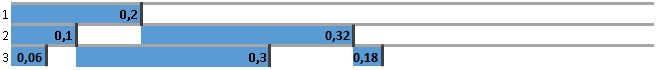
\includegraphics[scale=.75]{sections/images/third_logical_moment.jpg}
	\floatfoot{Example of the first three moments of an expansion.}%\footnotemark}
	\end{figure}
	%\footnotetext{Fonte: note}

Based on Figure \ref{fig:third_logical_moment}, the following observations can be extracted in relation to the first, second and third logical moments:
	\begin{description}
	   \item[First logical moment] The negation of the primordial logic to itself, subdivides it into two units, two sub-logics. Although these parts have different proportions, they express the same amounts of points or possibilities of change, since they are representations of the primordial logic, which \textit{ad infinitum}. The fractional part in blue represents the proportion of the logical negation to its unity.
	   \item[Second logical moment] It is generated by the negation of the two primordial sub-logics fractionated in the first logical moment, that is, the second logical moment is a negation of the first. In the impossibility of these sub-logics continuing to negate themselves, even for a brief instant, would make them unable to negate their two units of the whole and consequently to make it [be]. The fractional parts in blue represent the proportion of the logical negation to their respective units.
	   \item[Third logical moment] It follows from the negation of the second logical moment, just as the second logical moment follows from the negation of the first, and so on.
	\end{description}

With each negation or subnegation of the primordial logic, its new values are influenced by the adjacent values of the previous logical moment. In the figure \ref{fig:imposition_of_binomial_expansion}, the primordial logic negates itself by generating the first logical moment with the value [0,2].  In the second logical moment, its subdivisions are contained within the boundary imposed by the value of the first logical moment. The points of the third logical moment, for example, suffer the impositions of the values of the second logical moment, which in turn suffer the imposition of the first. Pascal's triangle has interesting properties about this relationship. 
	\begin{figure}[H]
	\caption{Logical expansion enforcement}
	\label{fig:imposition_of_binomial_expansion}
	\centering
	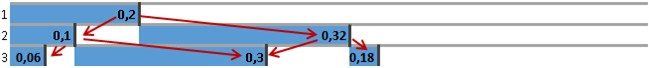
\includegraphics[scale=.75]{sections/images/imposition_of_binomial_expansion.jpg}
	\floatfoot{Cumulative imposition on descending logical moments.}%\footnotemark}
	\end{figure}
	%\footnotetext{Fonte: note}

In Pascal's triangle, Figure \ref{fig:pascal_triangle}, each number is the closest two numbers above added together. This number represents how many different possible paths lead to it. For example, the number [4] in Figure \ref{fig:pascal_triangle} represents the four different paths leading to it. The binomial coefficients found in Pascal's triangle represent only the amounts of impositions suffered by each value of a logical moment. Another interesting aspect of Pascal's triangle is the Fibonacci sequence, Figure \ref{fig:pascal_triangle_fibonacci} \cite{mathisfun_pascal_triangle}.
\enlargethispage{\baselineskip}
	\begin{figure}[H]
	\centering
		\begin{subfigure}[H]{0.47\linewidth}
		\centering
		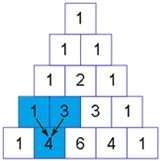
\includegraphics[width=.55\linewidth]{sections/images/pascal_triangle.jpg}
		\caption{}
		\label{fig:pascal_triangle}
		\end{subfigure}
	\hfill
		\begin{subfigure}[H]{0.47\linewidth}
		\centering
		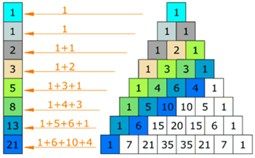
\includegraphics[width=.9\linewidth]{sections/images/pascal_triangle_fibonacci.jpg}
		\caption{}
		\label{fig:pascal_triangle_fibonacci}
		\end{subfigure}%
	\caption{Features of Pascal's triangle}
	\floatfoot{Source: MathsIsFun, 2019. \protect\footnotemark}
	\end{figure}
	\footnotetext{\url{www.mathsisfun.com/pascals-triangle.html}}
